\begin{python}
    self.dashboard <= w.label('Switch', typo='headline4', style=flex_title)
    self.dashboard <= w.switch(
        'Switch 1', checked=True, on_change=self.on_switch, id='my_swicth'
    )
    self.dashboard <= w.label(
        f'', id='for_switch', typo=f'body1', style=flex
    )


def on_switch(self, value):
    # value = self.widgets.get_value('my_swicth')
    document.select_one('#for_switch').html = f'Switch Changed: {value}'
\end{python}


\begin{figure}[H]
\begin{centering}
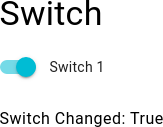
\includegraphics[scale=0.5]{Cap4/Figures/widgets/switch.png}
\par\end{centering}
\caption[Brython Radiant: Switch]{Brython Radiant: Switch.}
\label{fig:radiant_switch}
\end{figure}